\section{Исследовательская часть}

\subsection{Технические характеристики}

Замер процессорного времени был произведён на отладочной плате NUCLEO-F767ZI\cite{stm}, позволяющей запускать программы, написанные на языке \textit{MicroPython}\cite{python}.

Технические характеристики NUCLEO-F767ZI:
\begin{itemize}
    \item Разрядность шины данных --- 32 бита;
    \item Процессор --- Arm Cortex-M7;
    \item Объем ОЗУ --- 512 Кбайт;
\end{itemize}

\subsection{Замер процессорного времени}

Замер процессорного времени производился для строк, состоящих из случайных последовательностей символов длиной от одного до шести в кодировке $UTF-8$. При этом длина входных строк в рамках замера совпадает. Результатом для $i$-ой ($i=\overline{1,6}$) длины является среднее арифметическое показателей $n=15$ замеров. 

В таблице~\ref{table:timings} приведены результаты замеров процессорного времени работы алгоритмов нахождения расстояния Левенштейна (Л), и Дамерау~---~Левенштейна (ДЛ).

\begin{table}[htb]
\caption{\centering Результат замеров процессорного времени работы алгоритмов для строк длиной от 1 до 6 символов.}
\small
\centering\begin{tabular}{|c|c|c|c|c|}
    \hline
    \textbf{Length} & \textbf{Л (матрица)} & \textbf{ДЛ (матрица)} & \textbf{Л (рекурсия)} & \textbf{Л (рекурсия с кэшем)} \\
    \hline
    1 & 0.100097 & 0.097736 & 0.095129 & 0.347810 \\
    2 & 0.176366 & 0.204006 & 0.399600 & 1.138200 \\
    3 & 0.340942 & 0.394079 & 1.860301 & 2.702778 \\
    4 & 0.512742 & 0.631439 & 9.813755 & 4.151481 \\
    5 & 0.741701 & 0.947312 & 52.949607 & 6.649858 \\
    6 & 1.012530 & 1.341707 & 275.854151 & 9.246883 \\
    \hline
\end{tabular}
\label{table:timings}
\end{table}

На рисунке~\ref{fig:timings} представлены графики, построенные на основе табличных данных.

\begin{figure}[!htb]
    \centering
    \begin{minipage}[t]{0.55\textwidth}
        \centering
        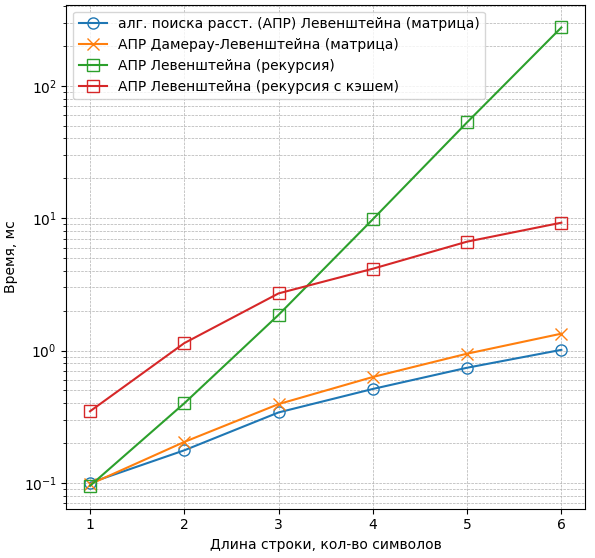
\includegraphics[width=\linewidth]{img/logarithmic.png}
        \caption*{а) Логарифмическая шкала}
    \end{minipage}

    \vspace{1em}

    \begin{minipage}[t]{0.55\textwidth}
        \centering
        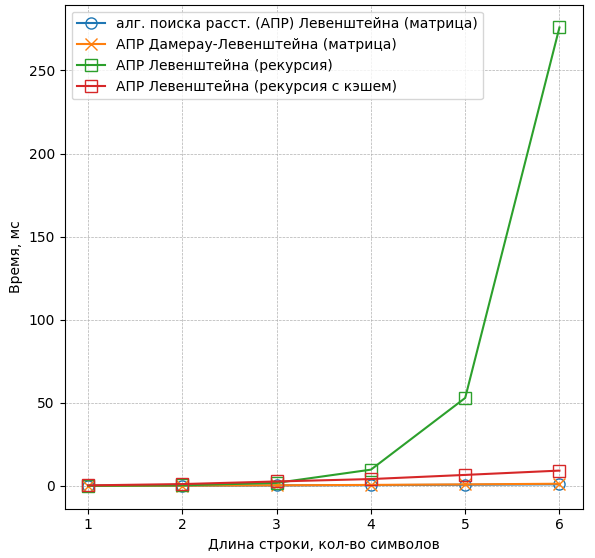
\includegraphics[width=\linewidth]{img/default.png}
        \caption*{б) Линейная шкала}
    \end{minipage}

    \caption{Зависимость процессорного времени работы алгоритмов от длины входных строк}
    \label{fig:timings}
\end{figure}

\newpage

\subsection{Оценка потребляемой памяти}

\subsubsection{Рекурсивный алгоритм Левенштейна}

Глубина рекурсии в рекурсивных алгоритмах нахождения расстояния Левенштейна в худшем случае будет составлять 

\begin{equation}
    (len(S_1) + len(S_2)).
\end{equation}

Также на каждом уровне создаются новые строки, что в худшем случае требует $sizeof(S_1) + sizeof(S_2)$ байт на каждом уровне рекурсии. При этом каждый рекурсивный вызов требует хранения двух локальных переменных длин входных строк. С учётом того, что в данном алгоритме используются три глобальные переменные $INSERT\_COST$, $DELETE\_COST$, $REPLACE\_COST$, которые в сумме занимают $3~\cdot~sizeof(int)$ байт, итоговый объем будет выражен формулой~\ref{eq:recur_lev}.

\begin{equation}
    \label{eq:recur_lev}
    (len(S_1) + len(S_2)) \cdot (sizeof(S_1) + sizeof(S_2) + 2 \cdot sizeof(int)) + 3 \cdot sizeof(int)
\end{equation}

\subsubsection{Рекурсивный алгоритм Левенштейна с мемоизацией}

При каждом рекурсивном вызове для хранения локальных переменных $length1$, $length2$ и $distance$ требуется $3 \cdot sizeof(int)$ байт, для хранения кортежа из двух целочисленных значений необходимо $key\_size = sizeof(tuple) + 2~\cdot~sizeof(int)$ байт, где $tuple$ - объект кортежа. 

Общее количество уникальных рекурсивных вызовов равно 

\begin{equation}
    \label{eq:recur_calls}
    (len(S_1) + 1)~\cdot~(len(S_2) + 1),
\end{equation}

а для хранения одной пары <<ключ-значение>>, где ключ --- кортеж из двух целых чисел, а значение --- одно целое число, требуется количество байт, вычисляемое по формуле~\ref{eq:key_value}.

\begin{equation}
    \label{eq:key_value}
    key\_value\_size = (key\_size + sizeof(int)).
\end{equation}

Тогда в худшем случае для словаря и его содержимого потребуется объем памяти, выраженный формулой~\ref{eq:dict_size}, где $dict$ --- объект словаря.

\begin{multline}
    \label{eq:dict_size}
    memo\_size = sizeof(dict) \\
    + (len(S_1) + 1) \cdot (len(S_2) + 1) \cdot key\_value\_size.
\end{multline}

С учётом того, что в данном алгоритме используются три глобальные переменные $INSERT\_COST$, $DELETE\_COST$, $REPLACE\_COST$, которые в сумме занимают $3~\cdot~sizeof(int)$ байт, итоговый объем памяти, необходимый в худшем случае, будет выражен формулой~\ref{eq:recur_memo_lev}.

\begin{multline}
    \label{eq:recur_memo_lev}
    ((len(S_1) + len(S_2)) \cdot (sizeof(S_1) + sizeof(S_2) \\
    + 3~\cdot~sizeof(int) + key\_size) \\
    + memo\_size + 3~\cdot~sizeof(int)).
\end{multline}

\subsubsection{Матричный алгоритм Левенштейна}

В данном алгоритме для хранения локальных переменных длин строк $S_1$, $S_2$ и параметра $cost$ необходимо $3~\cdot~sizeof(int)$ байт. Для хранения матрицы результатов $M$ необходимо $(len(S_1) + 1) \cdot (len(S_2) + 1) \cdot sizeof(int)$ байт. Также в данном алгоритме используются глобальные целочисленные переменные $INSERT\_COST$, $DELETE\_COST$, $REPLACE\_COST$, которые в сумме занимают $3~\cdot~sizeof(int)$ байт. Итоговый объем памяти выражен формулой~\ref{eq:dyn_lev}.

\begin{equation}
    \label{eq:dyn_lev}
    (len(S_1) + 1) \cdot (len(S_2) + 1) \cdot sizeof(int) + 6 \cdot sizeof(int)
\end{equation}

\subsubsection{Матричный алгоритм Дамерау~---~Левенштейна}

В данном алгоритме для хранения локальных переменных длин строк $S_1$, $S_2$ и параметра $cost$ необходимо $3~\cdot~sizeof(int)$ байт. Для хранения матрицы результатов $M$ необходимо $(sizeof(S_1) + 1) \cdot (sizeof(S_2) + 1) \cdot sizeof(int)$ байт. Также в данном алгоритме используются глобальные целочисленные переменные $INSERT\_COST$, $DELETE\_COST$, $REPLACE\_COST$ и $TRANSPOSITION\_COST$, которые в сумме занимают $4~\cdot~sizeof(int)$ байт. Итоговый объем памяти выражен формулой~\ref{eq:dyn_dam_lev}.

\begin{equation}
    \label{eq:dyn_dam_lev}
    (sizeof(S_1) + 1) \cdot (sizeof(S_2) + 1) \cdot sizeof(int) + 7 \cdot sizeof(int)
\end{equation}

\subsection{Вывод}

На основе результатов замера процессорного времени работы, можно сделать вывод, что матричные алгоритмы нахождения расстояний Левенштейна и Дамерау~---~Левенштейна имеют схожее время работы (в сравнении с рекурсивными алгоритмами разница между матричными алгоритмами крайне мала) и потребляемое количество памяти, т.~к. алгоритм нахождения расстояния Дамерау~---~Левенштейна использует всего на одну переменную больше ($TRANSPOSITION\_COST$). 

Простой рекурсивный алгоритм нахождения расстояния Левенштейна имеет худшее время работы. Также можно подтвердить, что мемоизация действительно даёт значительный прирост производительности, но при этом увеличивается количество потребляемой памяти, т.~к. необходимо хранить результаты предыдущих вызовов. 

Стоит отметить, что рекурсивные реализации имеют аппаратное ограничение, так как ввод длинных строк может привести к переполнению стека из-за множественных рекурсивных вызовов.

Выбор между алгоритмами нахождения расстояний Левенштейна и Дамерау~---~Левенштейна зависит от необходимости учёта операции транспозиции соседних символов.
